\chapter{Estado del arte}\label{cap:estado}

\section{Información de horarios académicos en la UGR}

La Universidad de Granada, al igual que muchas otras universidades descentraliza sus sedes, de modo que
cada una de ellas tiene su propio sistema de gestión de la información. En este sentido, las facultades cuentan
con una serie de sistemas de información propios que se encargan de la generación de horarios académicos,
asignación de aulas y profesores a los grupos tanto de teoría como de prácticas 
de las distintas titulaciones y asignaturas, etc. Y esta información a su vez se le facilita a la Universidad de Granada para la centralización de la información.
\newline\newline
Para acceder a la información de los horarios, los estudiantes y docentes pueden hacerlo de diferentes maneras:
\begin{itemize}
    \item A través de la página propia de su facultad. Poniéndo de ejemplo a la ETSIIT, debemos acceder a la página ``https://etsiit.ugr.es`` y buscar la información en la sección
          de ``Calendario de exámenes`` en caso de querer saber los días y rangos horarios de estos y visualizándolo con un pdf, o a ``Calendario académico y horarios`` y a ``Grado en Ingeniería Informática``
          en caso de querer saber los horarios de los diferentes grupos del grado, presentado todo ello en un pdf contenedor de alrededor de 40 tablas.
          \newline\newline
          De esta manera tendremos que buscar el año al que pertenece la asignatura de la que estamos matriculados y el grupo al que pertenecemos. De esta manera obtenemos su 
          franja horaria y aula, pero no profesor que imparte la asignatura.
          \newline\newline
          Sin embargo, el formato de las tablas cambia de un grado a otro, haciendo que el estudiante tenga que buscar la información de manera diferente en cada grado si está matriculado en más de uno, 
          y obteniendo información diferente. En el caso del grado de Administración y Dirección de Empresas por ejemplo, no se muestra el aula en la que se imparte la clase, pero sí las asignaturas bilingües, y
          los profesores que las imparten.
          \newline\newline
          Esta forma de visualización de horarios es muy poco eficiente, ya que el estudiante tiene que buscar la información de manera manual, es inconsistente entre grados, y no es accesible para personas con discapacidad visual.
          %% Comparación de horarios de diferentes grados ( 2 imágenes )
          %% Como se insertan dos imagenes en latex con un unico pie de foto -> 
          \newpage
            \begin{figure}[H]
                \centering
                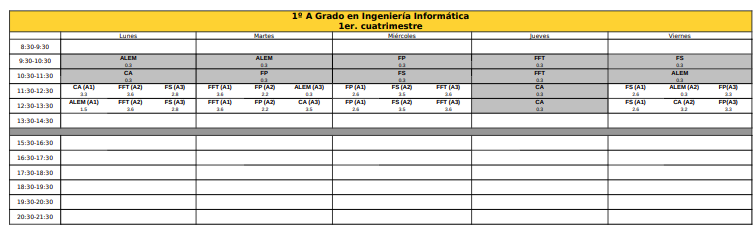
\includegraphics[width=0.8\textwidth]{figures/02_etsiit_horario.png}
                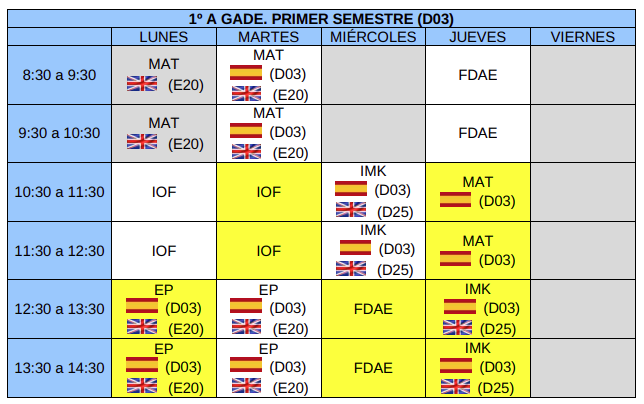
\includegraphics[width=0.8\textwidth]{figures/02_ade_horario.png}
                \caption{Comparación de horarios de diferentes grados: ETSIIT (arriba) y ADE (abajo).}
                \label{fig:horarios_comparacion}
            \end{figure}
          

    \item A través de la web ``https://grados.ugr.es/`` se puede buscar la información de los horarios de las asignaturas de los diferentes grados de la Universidad de Granada. Para ello debemos seleccionar rama de conocimiento, 
          grado, curso y asignatura. De esta manera obtenemos un horario semanal con las franjas horarias, aulas, profesores y fechas tanto de inicio como de fin. Este método nos proporcioan una interfaz estándar y más información, pero 
          también es más lento y tedioso para consultar por varias asignaturas o incluso grados.
    \item A través de las webs de cada departamento. Por ejemplo en la web de ``https://decsai.ugr.es/`` se puede consultar la información de las asignaturas o profesores de este.
          Ofrece información adicional como asignaturas que imparte ``x'' profesor y su horario de tutorías y docencia.
\end{itemize}

Además para acceder a la información de periodos de actividad docente, exámenes finales, periodos de evaluación de convocatorias ... se ha de acceder a la web de ``https://secretariageneral.ugr.es'' para consultar otro pdf.

En general la información de los horarios académicos de la Universidad de Granada es poco accesible, eficiente y consistente entre grados y facultades, lo que hace que el estudiante tenga que buscar la información de manera manual y tediosa.
Además no hay manera de consultar de manera sencilla un calendario personal que incluya tanto los horarios de las asignaturas como los exámenes y periodos de evaluación, entre otros.

\section{Comparación con otras instituciones}

\section{Acercamientos arquitectónicos}

\section{Tecnologías existentes}

